\documentclass[11pt,a4paper]{article}

% Essential packages for math
\usepackage{amsmath,amssymb,amsthm}
\usepackage{mathtools} 
\usepackage{bm}
 
% Page layout
\usepackage{geometry}
\geometry{margin=1in} 

% Graphics and colors
\usepackage{graphicx}
\usepackage{xcolor}
\usepackage{tikz}
\usepackage{pgfplots}
\pgfplotsset{compat=1.17}
\usetikzlibrary{shapes.geometric, arrows.meta, calc, patterns, positioning, decorations.pathmorphing, decorations.markings, 3d, shadows, backgrounds}

% Tables
\usepackage{booktabs}
\usepackage{multirow}
\usepackage{array}
\usepackage{longtable}
\usepackage{colortbl}
\usepackage{tabularx}

% Algorithms
\usepackage{algorithm}
\usepackage{algorithmicx}
\usepackage{algpseudocode}

% Code listings
\usepackage{listings}
\lstset{
    basicstyle=\ttfamily\small,
    breaklines=true,
    frame=single,
    numbers=left,
    numberstyle=\tiny,
    keywordstyle=\color{blue},
    commentstyle=\color{green!50!black},
    stringstyle=\color{red},
    showstringspaces=false
}

% References and links
\usepackage{hyperref}
\hypersetup{
    colorlinks=true,
    linkcolor=blue,
    citecolor=green,
    urlcolor=red
}

% Other useful packages
\usepackage{enumerate}
\usepackage{enumitem}
\usepackage{subcaption}
\usepackage{float}
\usepackage{wrapfig}
\usepackage{rotating}
\usepackage{footmisc}
\usepackage{fancyhdr}
\usepackage{lipsum}
\usepackage{soul} % for highlighting
\usepackage{ulem} % for underlining
\usepackage{cancel} % for canceling in equations
\usepackage{siunitx} % for SI units

% Chemistry
% \usepackage{chemfig}
\usepackage{mhchem}

% Advanced math
\usepackage{mathrsfs}
\usepackage{dsfont}

% Fancy headers
\pagestyle{fancy}
\fancyhf{}
\fancyhead[L]{\leftmark}
\fancyhead[R]{\thepage}
\fancyfoot[C]{Comprehensive LaTeX Test Document}

% Theorem environments
\theoremstyle{definition}
\newtheorem{definition}{Definition}[section]
\newtheorem{theorem}{Theorem}[section]
\newtheorem{lemma}[theorem]{Lemma}
\newtheorem{proposition}[theorem]{Proposition}
\newtheorem{corollary}[theorem]{Corollary}
\newtheorem{remark}{Remark}[section]
\newtheorem{example}{Example}[section]

% Custom commands
\newcommand{\E}{\mathbb{E}}
\newcommand{\R}{\mathbb{R}}
\newcommand{\N}{\mathcal{N}}
\newcommand{\C}{\mathbb{C}}
\newcommand{\Z}{\mathbb{Z}}
\newcommand{\Q}{\mathbb{Q}}
\newcommand{\KL}{\text{KL}}
\newcommand{\ELBO}{\text{ELBO}}
\DeclareMathOperator{\Var}{Var}
\DeclareMathOperator{\Cov}{Cov}
\DeclareMathOperator{\tr}{tr}
\DeclareMathOperator{\diag}{diag}

\title{\Huge \textbf{Comprehensive LaTeX Functionality Test}\\[0.5cm]
\Large Testing All Major LaTeX Features and Packages}
\author{GitHub Actions LaTeX Compiler Test\\[0.2cm]
\texttt{github-actions@compiler.test}}
\date{\today}

\begin{document}

\maketitle

\begin{abstract}
This document serves as a comprehensive test suite for LaTeX compilation, testing mathematics, algorithms, visualizations (TikZ/PGFPlots), tables, code listings, chemistry notation, 3D graphics, complex formatting, cross-references, footnotes, bibliography support, and various advanced LaTeX packages. This ensures the GitHub Actions workflow can handle real-world LaTeX documents.
\end{abstract}

\tableofcontents
\listoffigures
\listoftables
\newpage

\section{Advanced Mathematics}

\subsection{Complex Equations}

Testing multi-line equations with alignment:

\begin{align}
    \oint_C \mathbf{F} \cdot d\mathbf{r} &= \iint_S (\nabla \times \mathbf{F}) \cdot d\mathbf{S} \label{eq:stokes} \\
    \nabla \cdot \mathbf{E} &= \frac{\rho}{\epsilon_0} \label{eq:gauss} \\
    \nabla \times \mathbf{B} &= \mu_0\mathbf{J} + \mu_0\epsilon_0\frac{\partial \mathbf{E}}{\partial t} \label{eq:ampere}
\end{align}

Testing equation cancellation and highlighting:
\begin{equation}
    \cancel{\frac{x^2}{x}} \cdot \frac{y^3}{y^2} = x \cdot y
\end{equation}

\subsection{Matrix Operations}

Block matrices and determinants:
\begin{equation}
    \det\begin{bmatrix}
        \mathbf{A} & \mathbf{B} \\
        \mathbf{C} & \mathbf{D}
    \end{bmatrix} = \det(\mathbf{A})\det(\mathbf{D} - \mathbf{C}\mathbf{A}^{-1}\mathbf{B})
\end{equation}

Eigenvector equation:
\begin{equation}
    \mathbf{A}\mathbf{v} = \lambda\mathbf{v} \implies \det(\mathbf{A} - \lambda\mathbf{I}) = 0
\end{equation}

\subsection{Special Functions}

Testing special mathematical symbols:
\begin{align}
    \Gamma(n) &= (n-1)! \quad \text{for } n \in \mathbb{N}^+ \\
    \zeta(s) &= \sum_{n=1}^{\infty} \frac{1}{n^s} \quad \text{for } \Re(s) > 1 \\
    \mathcal{F}\{f(t)\} &= \int_{-\infty}^{\infty} f(t)e^{-2\pi i \xi t}\,dt
\end{align}

\subsection{Advanced Calculus}

Multivariable calculus with gradients:
\begin{equation}
    \nabla f = \frac{\partial f}{\partial x}\mathbf{i} + \frac{\partial f}{\partial y}\mathbf{j} + \frac{\partial f}{\partial z}\mathbf{k}
\end{equation}

Chain rule in multiple dimensions:
\begin{equation}
    \frac{\partial z}{\partial u} = \frac{\partial z}{\partial x}\frac{\partial x}{\partial u} + \frac{\partial z}{\partial y}\frac{\partial y}{\partial u}
\end{equation}

\subsection{Statistical Distributions}

\begin{definition}[Multivariate Gaussian]
A $d$-dimensional multivariate Gaussian distribution is defined as:
\begin{equation}
    p(\mathbf{x}) = \frac{1}{(2\pi)^{d/2}|\mathbf{\Sigma}|^{1/2}} \exp\left(-\frac{1}{2}(\mathbf{x}-\bm{\mu})^T\mathbf{\Sigma}^{-1}(\mathbf{x}-\bm{\mu})\right)
\end{equation}
\end{definition}

\subsection{Set Theory and Logic}

Testing logical symbols:
\begin{align}
    \forall x \in \mathbb{R}, \exists y \in \mathbb{R} &: x < y \\
    A \cap B &= \{x : x \in A \land x \in B\} \\
    A \cup B &= \{x : x \in A \lor x \in B\} \\
    A \setminus B &= \{x : x \in A \land x \notin B\}
\end{align}

\section{Chemistry Notation}

\subsection{Chemical Formulas}

Using mhchem package:
\begin{equation}
    \ce{CO2 + C -> 2CO}
\end{equation}

\begin{equation}
    \ce{Zn^2+ <=>[+ 2OH-][+ 2H+] $\underset{\text{amphoteric hydroxide}}{\ce{Zn(OH)2 v}}$ <=>[+ 2OH-][+ 2H+] $\underset{\text{tetrahydroxozincate}}{\ce{[Zn(OH)4]^2-}}$}
\end{equation}

Reaction with arrows:
\begin{equation}
    \ce{H2O <=> H+ + OH-}
\end{equation}

\subsection{Structural Chemistry}

Using chemfig package:
\begin{center}
\chemfig{H-C(-[2]H)(-[6]H)-C(=[1]O)-O-H}
\quad (Acetic Acid)
\end{center}

\begin{center}
\chemfig{*6(-=-(-NH_2)=-=)}
\quad (Aniline)
\end{center}

\section{Units and Measurements}

Using siunitx package for proper SI units:

\begin{itemize}
    \item Temperature: \SI{25}{\celsius} or \SI{298.15}{\kelvin}
    \item Energy: \SI{6.626e-34}{\joule\second}
    \item Speed: \SI{3e8}{\meter\per\second}
    \item Concentration: \SI{1.5}{\mol\per\liter}
    \item Angle: \ang{45;30;30}
\end{itemize}

\section{Complex Tables}

\subsection{Multi-row and Multi-column Tables}

\begin{table}[H]
\centering
\caption{Advanced Table with Multiple Features}
\label{tab:advanced}
\begin{tabular}{|l|c|c|c|c|}
\hline
\rowcolor{gray!30}
\multirow{2}{*}{\textbf{Model}} & \multicolumn{2}{c|}{\textbf{Accuracy (\%)}} & \multicolumn{2}{c|}{\textbf{Time (ms)}} \\
\cline{2-5}
\rowcolor{gray!30}
 & Train & Test & Forward & Backward \\
\hline
ResNet-50 & 95.2 & 92.8 & 23.4 & 45.6 \\
\rowcolor{blue!10}
VGG-16 & 93.8 & 91.2 & 34.5 & 67.8 \\
MobileNet & 89.4 & 87.6 & 12.3 & 18.9 \\
\rowcolor{green!10}
EfficientNet & \textbf{96.7} & \textbf{94.3} & 18.2 & 32.1 \\
\hline
\end{tabular}
\end{table}

\subsection{Long Table Spanning Multiple Pages}

\begin{longtable}{|l|r|r|p{6cm}|}
\caption{Long Table Example} \label{tab:long} \\
\hline
\textbf{ID} & \textbf{Value 1} & \textbf{Value 2} & \textbf{Description} \\
\hline
\endfirsthead

\multicolumn{4}{c}%
{{\tablename\ \thetable{} -- continued from previous page}} \\
\hline
\textbf{ID} & \textbf{Value 1} & \textbf{Value 2} & \textbf{Description} \\
\hline
\endhead

\hline \multicolumn{4}{r}{{Continued on next page}} \\
\endfoot

\hline
\endlastfoot

1 & 123 & 456 & This is a long description to test paragraph wrapping in tables \\
2 & 789 & 012 & Another entry with substantial text content \\
3 & 345 & 678 & Testing multi-line cell content in longtable environment \\
4 & 901 & 234 & More data rows for comprehensive testing \\
5 & 567 & 890 & Additional entries to demonstrate pagination \\
\end{longtable}

\section{Advanced TikZ Graphics}

\subsection{3D Graphics}

\begin{figure}[H]
\centering
\begin{tikzpicture}[scale=1.5]
    % 3D coordinate system
    \draw[->] (0,0,0) -- (4,0,0) node[right] {$x$};
    \draw[->] (0,0,0) -- (0,4,0) node[above] {$y$};
    \draw[->] (0,0,0) -- (0,0,4) node[below left] {$z$};
    
    % 3D surface representation
    \foreach \z in {0,0.5,...,3}{
        \draw[blue, opacity=0.3] plot[domain=0:3, smooth] (\x, {sin(\x*180/3.14)*exp(-\z/3)}, \z);
    }
    
    \node at (2,-1,-1) {3D Damped Sine Wave};
\end{tikzpicture}
\caption{3D Graphics with TikZ}
\label{fig:3d}
\end{figure}

\subsection{Neural Network Diagram}

\begin{figure}[H]
\centering
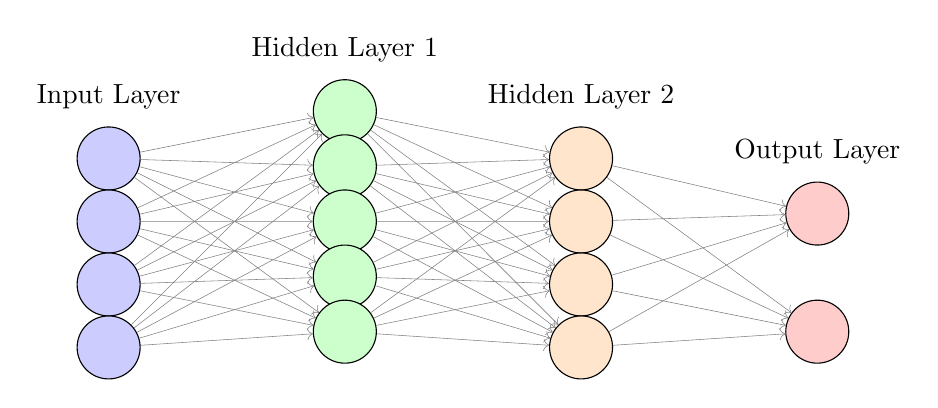
\begin{tikzpicture}[
    node distance=2cm,
    neuron/.style={circle, draw, minimum size=0.8cm, fill=blue!20},
    layer/.style={rectangle, draw, minimum width=1.5cm, minimum height=3cm, fill=gray!20}
]
    % Input layer
    \foreach \i in {1,2,3,4} {
        \node[neuron] (input\i) at (0, -\i*0.8) {};
    }
    \node[above=0.1cm of input1] {Input Layer};
    
    % Hidden layer 1
    \foreach \i in {1,2,3,4,5} {
        \node[neuron, fill=green!20] (hidden1\i) at (3, -\i*0.7+0.5) {};
    }
    \node[above=0.1cm of hidden11] {Hidden Layer 1};
    
    % Hidden layer 2
    \foreach \i in {1,2,3,4} {
        \node[neuron, fill=orange!20] (hidden2\i) at (6, -\i*0.8) {};
    }
    \node[above=0.1cm of hidden21] {Hidden Layer 2};
    
    % Output layer
    \foreach \i in {1,2} {
        \node[neuron, fill=red!20] (output\i) at (9, -\i*1.5) {};
    }
    \node[above=0.1cm of output1] {Output Layer};
    
    % Connections (sample)
    \foreach \i in {1,2,3,4} {
        \foreach \j in {1,2,3,4,5} {
            \draw[->, very thin, gray] (input\i) -- (hidden1\j);
        }
    }
    
    \foreach \i in {1,2,3,4,5} {
        \foreach \j in {1,2,3,4} {
            \draw[->, very thin, gray] (hidden1\i) -- (hidden2\j);
        }
    }
    
    \foreach \i in {1,2,3,4} {
        \foreach \j in {1,2} {
            \draw[->, very thin, gray] (hidden2\i) -- (output\j);
        }
    }
\end{tikzpicture}
\caption{Deep Neural Network Architecture}
\label{fig:nn}
\end{figure}

\subsection{Flowchart}

\begin{figure}[H]
\centering
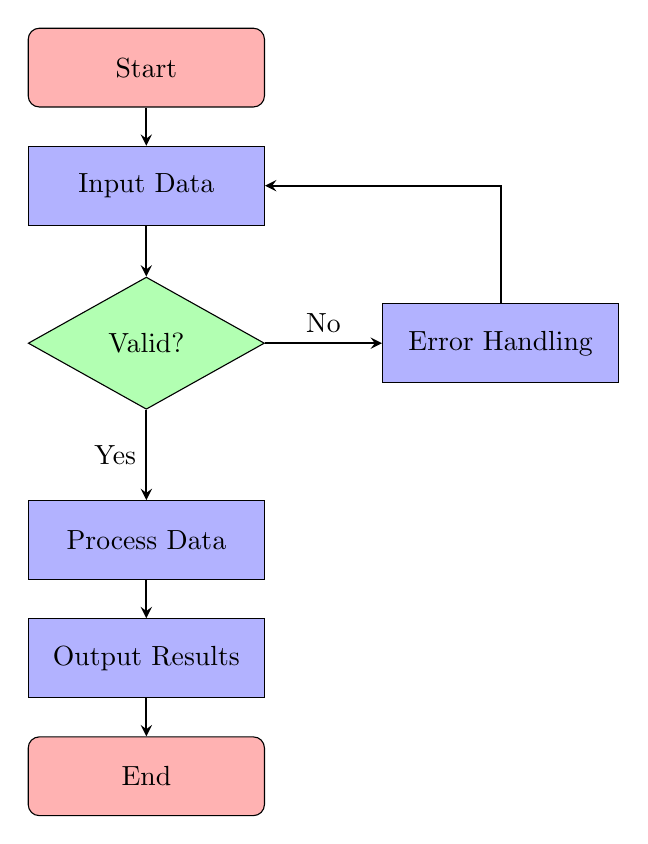
\begin{tikzpicture}[
    node distance=1.5cm,
    startstop/.style={rectangle, rounded corners, minimum width=3cm, minimum height=1cm, text centered, draw=black, fill=red!30},
    process/.style={rectangle, minimum width=3cm, minimum height=1cm, text centered, draw=black, fill=blue!30},
    decision/.style={diamond, minimum width=3cm, minimum height=1cm, text centered, draw=black, fill=green!30},
    arrow/.style={thick,->,>=stealth}
]
    \node (start) [startstop] {Start};
    \node (input) [process, below of=start] {Input Data};
    \node (check) [decision, below of=input, yshift=-0.5cm] {Valid?};
    \node (process1) [process, below of=check, yshift=-1cm] {Process Data};
    \node (process2) [process, right of=check, xshift=3cm] {Error Handling};
    \node (output) [process, below of=process1] {Output Results};
    \node (stop) [startstop, below of=output] {End};
    
    \draw [arrow] (start) -- (input);
    \draw [arrow] (input) -- (check);
    \draw [arrow] (check) -- node[anchor=east] {Yes} (process1);
    \draw [arrow] (check) -- node[anchor=south] {No} (process2);
    \draw [arrow] (process2) |- (input);
    \draw [arrow] (process1) -- (output);
    \draw [arrow] (output) -- (stop);
\end{tikzpicture}
\caption{Data Processing Flowchart}
\label{fig:flowchart}
\end{figure}

\subsection{Complex PGFPlots}

\begin{figure}[H]
\centering
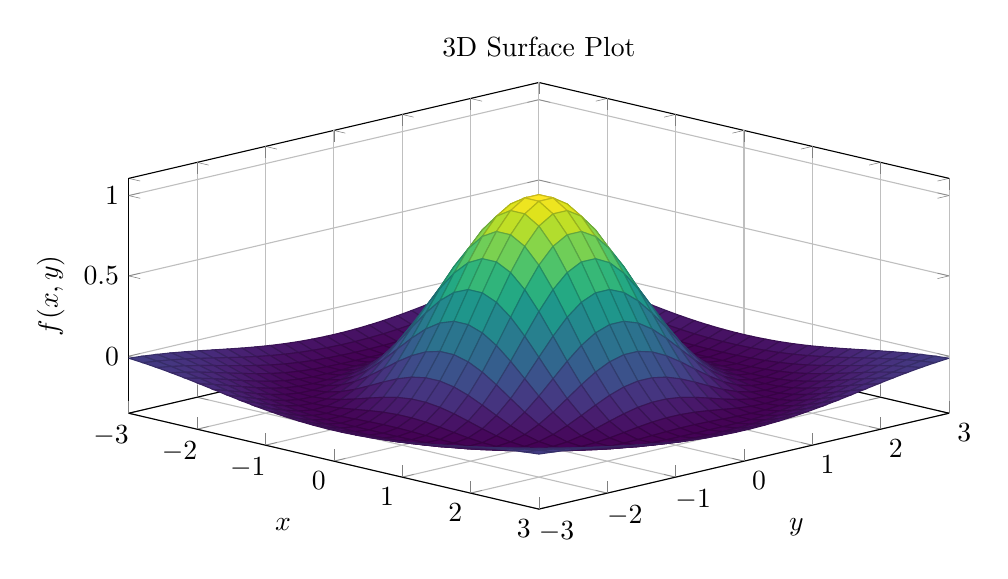
\begin{tikzpicture}
\begin{axis}[
    width=12cm,
    height=7cm,
    xlabel={$x$},
    ylabel={$y$},
    zlabel={$f(x,y)$},
    title={3D Surface Plot},
    view={45}{30},
    grid=major,
    colormap/viridis
]
\addplot3[
    surf,
    domain=-3:3,
    domain y=-3:3,
    samples=30,
] {exp(-(x^2+y^2)/5) * cos(deg(sqrt(x^2+y^2)))};
\end{axis}
\end{tikzpicture}
\caption{3D Surface Plot using PGFPlots}
\label{fig:3dplot}
\end{figure}

\begin{figure}[H]
\centering
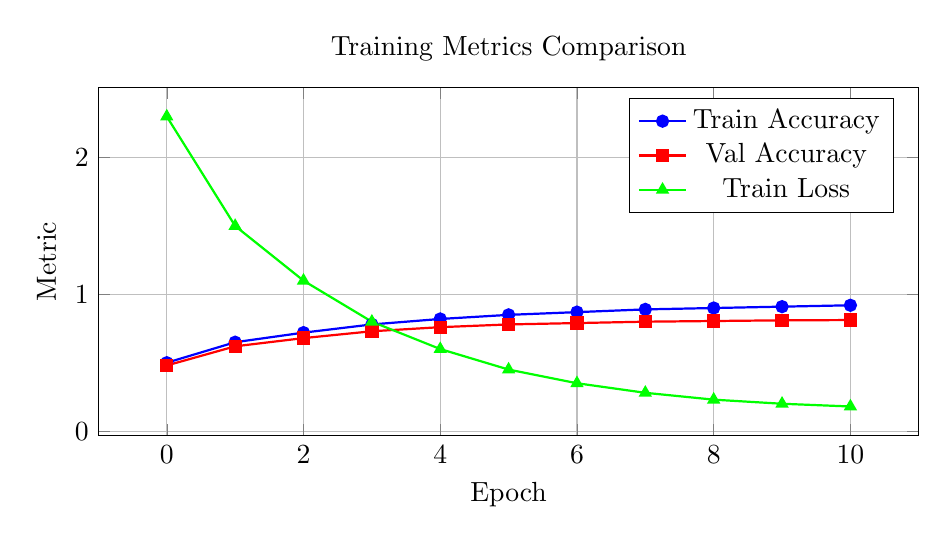
\begin{tikzpicture}
\begin{axis}[
    width=12cm,
    height=6cm,
    xlabel={Epoch},
    ylabel={Metric},
    legend pos=north east,
    grid=major,
    title={Training Metrics Comparison}
]
% Training accuracy
\addplot[blue, thick, mark=*] coordinates {
    (0,0.5) (1,0.65) (2,0.72) (3,0.78) (4,0.82) 
    (5,0.85) (6,0.87) (7,0.89) (8,0.90) (9,0.91) (10,0.92)
};
\addlegendentry{Train Accuracy}

% Validation accuracy
\addplot[red, thick, mark=square*] coordinates {
    (0,0.48) (1,0.62) (2,0.68) (3,0.73) (4,0.76) 
    (5,0.78) (6,0.79) (7,0.80) (8,0.805) (9,0.81) (10,0.812)
};
\addlegendentry{Val Accuracy}

% Training loss
\addplot[green, thick, mark=triangle*] coordinates {
    (0,2.3) (1,1.5) (2,1.1) (3,0.8) (4,0.6) 
    (5,0.45) (6,0.35) (7,0.28) (8,0.23) (9,0.20) (10,0.18)
};
\addlegendentry{Train Loss}
\end{axis}
\end{tikzpicture}
\caption{Multi-metric Training Curves}
\label{fig:metrics}
\end{figure}

\section{Advanced Algorithms}

\subsection{Recursive Algorithm}

\begin{algorithm}[H]
\caption{Merge Sort}
\label{alg:mergesort}
\begin{algorithmic}[1]
\Function{MergeSort}{$A, p, r$}
    \If{$p < r$}
        \State $q \gets \lfloor (p + r) / 2 \rfloor$
        \State \Call{MergeSort}{$A, p, q$}
        \State \Call{MergeSort}{$A, q+1, r$}
        \State \Call{Merge}{$A, p, q, r$}
    \EndIf
\EndFunction
\State
\Function{Merge}{$A, p, q, r$}
    \State $n_1 \gets q - p + 1$
    \State $n_2 \gets r - q$
    \State Create arrays $L[1..n_1+1]$ and $R[1..n_2+1]$
    \For{$i \gets 1$ \textbf{to} $n_1$}
        \State $L[i] \gets A[p + i - 1]$
    \EndFor
    \For{$j \gets 1$ \textbf{to} $n_2$}
        \State $R[j] \gets A[q + j]$
    \EndFor
    \State $L[n_1+1] \gets \infty$
    \State $R[n_2+1] \gets \infty$
    \State $i \gets 1$, $j \gets 1$
    \For{$k \gets p$ \textbf{to} $r$}
        \If{$L[i] \leq R[j]$}
            \State $A[k] \gets L[i]$
            \State $i \gets i + 1$
        \Else
            \State $A[k] \gets R[j]$
            \State $j \gets j + 1$
        \EndIf
    \EndFor
\EndFunction
\end{algorithmic}
\end{algorithm}

\subsection{Dynamic Programming}

\begin{algorithm}[H]
\caption{Longest Common Subsequence}
\label{alg:lcs}
\begin{algorithmic}[1]
\Function{LCS}{$X, Y$}
    \State $m \gets |X|$, $n \gets |Y|$
    \State Create table $c[0..m, 0..n]$
    \For{$i \gets 0$ \textbf{to} $m$}
        \State $c[i, 0] \gets 0$
    \EndFor
    \For{$j \gets 0$ \textbf{to} $n$}
        \State $c[0, j] \gets 0$
    \EndFor
    \For{$i \gets 1$ \textbf{to} $m$}
        \For{$j \gets 1$ \textbf{to} $n$}
            \If{$X[i] = Y[j]$}
                \State $c[i, j] \gets c[i-1, j-1] + 1$
            \Else
                \State $c[i, j] \gets \max(c[i-1, j], c[i, j-1])$
            \EndIf
        \EndFor
    \EndFor
    \State \Return $c[m, n]$
\EndFunction
\end{algorithmic}
\end{algorithm}

\section{Code Listings in Multiple Languages}

\subsection{Python Implementation}

\begin{lstlisting}[language=Python, caption=Matrix Multiplication in NumPy]
import numpy as np
from typing import Tuple

def matrix_multiply(A: np.ndarray, B: np.ndarray) -> np.ndarray:
    """
    Multiply two matrices using NumPy.
    
    Args:
        A: First matrix of shape (m, n)
        B: Second matrix of shape (n, p)
    
    Returns:
        Product matrix of shape (m, p)
    """
    if A.shape[1] != B.shape[0]:
        raise ValueError("Incompatible dimensions for matrix multiplication")
    
    # Using @ operator for matrix multiplication
    C = A @ B
    
    # Alternative: using np.matmul or np.dot
    # C = np.matmul(A, B)
    # C = np.dot(A, B)
    
    return C

# Example usage
if __name__ == "__main__":
    A = np.random.randn(100, 50)
    B = np.random.randn(50, 75)
    C = matrix_multiply(A, B)
    print(f"Result shape: {C.shape}")
\end{lstlisting}

\subsection{C++ Implementation}

\begin{lstlisting}[language=C++, caption=Binary Search Tree in C++]
#include <iostream>
#include <memory>

template<typename T>
class BST {
private:
    struct Node {
        T data;
        std::unique_ptr<Node> left;
        std::unique_ptr<Node> right;
        
        Node(T val) : data(val), left(nullptr), right(nullptr) {}
    };
    
    std::unique_ptr<Node> root;
    
    void insertHelper(std::unique_ptr<Node>& node, T value) {
        if (!node) {
            node = std::make_unique<Node>(value);
            return;
        }
        if (value < node->data) {
            insertHelper(node->left, value);
        } else {
            insertHelper(node->right, value);
        }
    }

public:
    BST() : root(nullptr) {}
    
    void insert(T value) {
        insertHelper(root, value);
    }
    
    bool search(T value) const {
        Node* current = root.get();
        while (current) {
            if (value == current->data) return true;
            current = (value < current->data) ? 
                      current->left.get() : current->right.get();
        }
        return false;
    }
};
\end{lstlisting}

\subsection{JavaScript Implementation}

\begin{lstlisting}[language=Java, caption=Promises and Async in JavaScript]
// Async/await example with error handling
async function fetchUserData(userId) {
    try {
        const response = await fetch(`/api/users/${userId}`);
        if (!response.ok) {
            throw new Error(`HTTP error! status: ${response.status}`);
        }
        const data = await response.json();
        return data;
    } catch (error) {
        console.error('Failed to fetch user data:', error);
        throw error;
    }
}

// Promise chain example
function processData(data) {
    return new Promise((resolve, reject) => {
        setTimeout(() => {
            if (data && data.length > 0) {
                resolve(data.map(item => item * 2));
            } else {
                reject(new Error('Invalid data'));
            }
        }, 1000);
    });
}

// Usage
fetchUserData(123)
    .then(user => console.log('User:', user))
    .catch(err => console.error('Error:', err));
\end{lstlisting}

\section{Text Formatting Features}

\subsection{Various Text Styles}

This paragraph demonstrates \textbf{bold text}, \textit{italic text}, \texttt{monospace text}, \underline{underlined text}, and \textsc{Small Caps Text}.

We can also use \hl{highlighted text}, \st{strikethrough text}, and \dashuline{dashed underline}.

\subsection{Special Characters and Symbols}

Common symbols: \% \$ \& \# \_ \{ \} \textbackslash{} \~{} \^{}

Quotation marks: ``double quotes'' and `single quotes'

Em-dash: This is an example---note the three hyphens.

Ellipsis: This is how it works\ldots

\subsection{Footnotes}

This is a sentence with a footnote\footnote{This is the footnote text at the bottom of the page.}. Here's another one\footnote{Second footnote for testing multiple footnotes.}.

\subsection{Lists with Custom Formatting}

\begin{enumerate}[label=(\Roman*)]
    \item First item with Roman numerals
    \item Second item
    \begin{enumerate}[label=(\alph*)]
        \item Nested item with letters
        \item Another nested item
    \end{enumerate}
    \item Third item
\end{enumerate}

\begin{itemize}[label=$\triangleright$]
    \item Custom bullet point
    \item Another custom bullet
    \begin{itemize}[label=$\circ$]
        \item Nested with circles
        \item More nesting
    \end{itemize}
\end{itemize}

\section{Wrap Figures and Side Captions}

\begin{wrapfigure}{r}{0.4\textwidth}
\centering
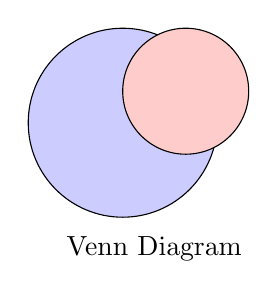
\begin{tikzpicture}[scale=0.8]
    \draw[fill=blue!20] (0,0) circle (1.5);
    \draw[fill=red!20] (1,0.5) circle (1);
    \node at (0.5,-2) {Venn Diagram};
\end{tikzpicture}
\caption{Wrapped figure example}
\label{fig:wrap}
\end{wrapfigure}

This text wraps around the figure on the right. \lipsum[1]

The figure demonstrates the wrapfig package functionality, which allows text to flow around figures. This is particularly useful for documents with many small figures that don't need to take up the full width of the page.

\clearpage

\section{Subfigures and Complex Layouts}

\begin{figure}[H]
\centering
\begin{subfigure}[b]{0.45\textwidth}
    \centering
    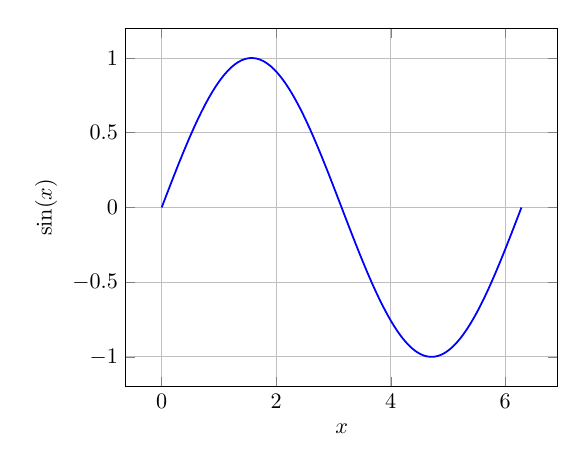
\begin{tikzpicture}[scale=0.8]
        \begin{axis}[
            domain=0:2*pi,
            samples=100,
            xlabel=$x$,
            ylabel=$\sin(x)$,
            grid=major
        ]
        \addplot[blue, thick] {sin(deg(x))};
        \end{axis}
    \end{tikzpicture}
    \caption{Sine function}
    \label{fig:sub1}
\end{subfigure}
\hfill
\begin{subfigure}[b]{0.45\textwidth}
    \centering
    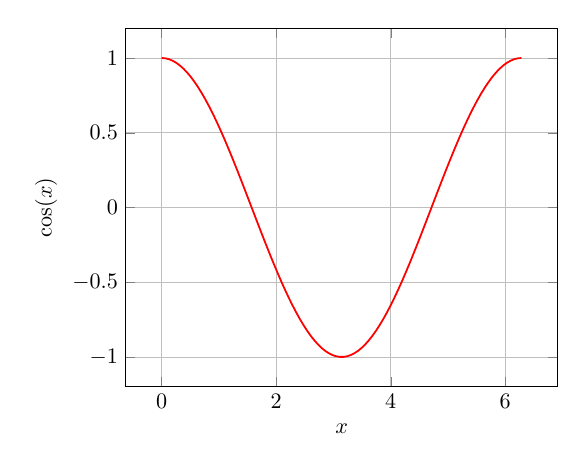
\begin{tikzpicture}[scale=0.8]
        \begin{axis}[
            domain=0:2*pi,
            samples=100,
            xlabel=$x$,
            ylabel=$\cos(x)$,
            grid=major
        ]
        \addplot[red, thick] {cos(deg(x))};
        \end{axis}
    \end{tikzpicture}
    \caption{Cosine function}
    \label{fig:sub2}
\end{subfigure}

\vspace{0.5cm}

\begin{subfigure}[b]{0.45\textwidth}
    \centering
    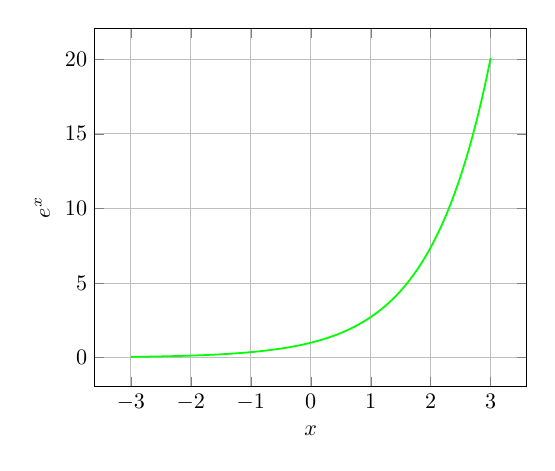
\begin{tikzpicture}[scale=0.8]
        \begin{axis}[
            domain=-3:3,
            samples=100,
            xlabel=$x$,
            ylabel=$e^x$,
            grid=major
        ]
        \addplot[green, thick] {exp(x)};
        \end{axis}
    \end{tikzpicture}
    \caption{Exponential function}
    \label{fig:sub3}
\end{subfigure}
\hfill
\begin{subfigure}[b]{0.45\textwidth}
    \centering
    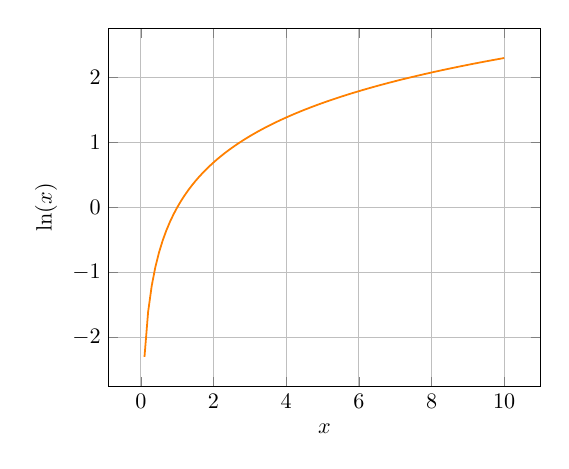
\begin{tikzpicture}[scale=0.8]
        \begin{axis}[
            domain=0.1:10,
            samples=100,
            xlabel=$x$,
            ylabel=$\ln(x)$,
            grid=major
        ]
        \addplot[orange, thick] {ln(x)};
        \end{axis}
    \end{tikzpicture}
    \caption{Natural logarithm}
    \label{fig:sub4}
\end{subfigure}
\caption{Common mathematical functions}
\label{fig:functions}
\end{figure}

\section{Rotated Content}

\subsection{Sideways Table}

\begin{sidewaystable}
\centering
\caption{Wide Table in Landscape Orientation}
\label{tab:sideways}
\begin{tabular}{lcccccccccc}
\toprule
\textbf{Method} & \textbf{Year} & \textbf{Acc.} & \textbf{Prec.} & \textbf{Rec.} & \textbf{F1} & \textbf{AUC} & \textbf{Time} & \textbf{Mem.} & \textbf{Params} & \textbf{FLOPs} \\
\midrule
CNN-Basic & 2015 & 87.3 & 85.2 & 86.1 & 85.6 & 0.91 & 12.3 & 2.1 & 5M & 1.2G \\
ResNet-50 & 2016 & 92.1 & 91.8 & 90.5 & 91.1 & 0.95 & 23.4 & 4.5 & 25M & 4.1G \\
VGG-16 & 2015 & 89.7 & 88.9 & 89.2 & 89.0 & 0.93 & 34.5 & 6.8 & 138M & 15.5G \\
MobileNet & 2017 & 88.2 & 87.5 & 88.1 & 87.8 & 0.92 & 12.3 & 1.2 & 4M & 0.6G \\
EfficientNet & 2019 & 94.3 & 93.8 & 94.1 & 94.0 & 0.97 & 18.2 & 2.8 & 7M & 1.8G \\
Transformer & 2020 & 95.8 & 95.2 & 95.6 & 95.4 & 0.98 & 45.6 & 8.9 & 86M & 12.3G \\
\bottomrule
\end{tabular}
\end{sidewaystable}

\section{Cross-References and Labels}

This document contains numerous cross-references. For example:
\begin{itemize}
    \item Equation \ref{eq:stokes} shows Stokes' theorem
    \item Figure \ref{fig:3d} demonstrates 3D graphics
    \item Table \ref{tab:advanced} contains multi-row data
    \item Algorithm \ref{alg:mergesort} implements merge sort
    \item Section \ref{sec:theorems} discusses advanced theorems
\end{itemize}

\section{Advanced Theorems and Proofs}
\label{sec:theorems}

\begin{theorem}[Cauchy-Schwarz Inequality]
For any vectors $\mathbf{u}, \mathbf{v} \in \mathbb{R}^n$:
\begin{equation}
    |\langle \mathbf{u}, \mathbf{v} \rangle| \leq \|\mathbf{u}\| \cdot \|\mathbf{v}\|
\end{equation}
\end{theorem}

\begin{proof}
Consider the quadratic function:
\begin{equation}
    f(t) = \|\mathbf{u} - t\mathbf{v}\|^2 = \langle \mathbf{u} - t\mathbf{v}, \mathbf{u} - t\mathbf{v} \rangle
\end{equation}

Expanding:
\begin{align}
    f(t) &= \langle \mathbf{u}, \mathbf{u} \rangle - 2t\langle \mathbf{u}, \mathbf{v} \rangle + t^2\langle \mathbf{v}, \mathbf{v} \rangle \\
    &= \|\mathbf{u}\|^2 - 2t\langle \mathbf{u}, \mathbf{v} \rangle + t^2\|\mathbf{v}\|^2
\end{align}

Since $f(t) \geq 0$ for all $t$, the discriminant must be non-positive:
\begin{equation}
    4\langle \mathbf{u}, \mathbf{v} \rangle^2 - 4\|\mathbf{u}\|^2\|\mathbf{v}\|^2 \leq 0
\end{equation}

Therefore:
\begin{equation}
    \langle \mathbf{u}, \mathbf{v} \rangle^2 \leq \|\mathbf{u}\|^2\|\mathbf{v}\|^2
\end{equation}

Taking square roots of both sides completes the proof.
\end{proof}

\begin{lemma}[Triangle Inequality]
For any vectors $\mathbf{u}, \mathbf{v} \in \mathbb{R}^n$:
\begin{equation}
    \|\mathbf{u} + \mathbf{v}\| \leq \|\mathbf{u}\| + \|\mathbf{v}\|
\end{equation}
\end{lemma}

\begin{corollary}
The reverse triangle inequality also holds:
\begin{equation}
    |\|\mathbf{u}\| - \|\mathbf{v}\|| \leq \|\mathbf{u} - \mathbf{v}\|
\end{equation}
\end{corollary}

\begin{example}[Computing Inner Products]
Let $\mathbf{u} = (1, 2, 3)$ and $\mathbf{v} = (4, 5, 6)$. Then:
\begin{align}
    \langle \mathbf{u}, \mathbf{v} \rangle &= 1 \cdot 4 + 2 \cdot 5 + 3 \cdot 6 = 32 \\
    \|\mathbf{u}\| &= \sqrt{1^2 + 2^2 + 3^2} = \sqrt{14} \\
    \|\mathbf{v}\| &= \sqrt{4^2 + 5^2 + 6^2} = \sqrt{77}
\end{align}

Verifying Cauchy-Schwarz: $|32| \leq \sqrt{14} \cdot \sqrt{77} = \sqrt{1078} \approx 32.83$ \checkmark
\end{example}

\begin{remark}
The Cauchy-Schwarz inequality is fundamental in functional analysis and has applications in machine learning, particularly in kernel methods and similarity measures.
\end{remark}

\section{Advanced Equation Environments}

\subsection{Cases and Piecewise Functions}

\begin{equation}
    f(x) = \begin{cases}
        x^2 & \text{if } x \geq 0 \\
        -x^2 & \text{if } x < 0
    \end{cases}
\end{equation}

\subsection{Matrices with Special Formatting}

Block matrix:
\begin{equation}
    \mathbf{M} = \left[\begin{array}{c|c}
        \mathbf{A} & \mathbf{B} \\
        \hline
        \mathbf{C} & \mathbf{D}
    \end{array}\right]
\end{equation}

Augmented matrix for linear systems:
\begin{equation}
    \left[\begin{array}{ccc|c}
        1 & 2 & 3 & 4 \\
        5 & 6 & 7 & 8 \\
        9 & 10 & 11 & 12
    \end{array}\right]
\end{equation}

\subsection{Multi-line Equations with Annotations}

\begin{align}
    \frac{d}{dx}\left[\int_a^x f(t)\,dt\right] &= f(x) \tag{Fundamental Theorem} \\
    \int_a^b f(x)\,dx &= F(b) - F(a) \tag{Evaluation} \\
    \int u\,dv &= uv - \int v\,du \tag{Integration by Parts}
\end{align}

\section{Circuit Diagrams with CircuiTikZ}

Unfortunately, CircuiTikZ requires additional setup. Here's a basic electrical circuit using standard TikZ:

\begin{figure}[H]
\centering
\begin{tikzpicture}[scale=1.2]
    % Resistors
    \draw (0,0) to[short] (0,2);
    \draw (0,2) -- (2,2);
    \draw[thick] (2,2) -- (2.5,2.2) -- (3,2) -- (3.5,2.2) -- (4,2);
    \node at (3,2.5) {$R_1$};
    
    \draw (4,2) -- (6,2);
    \draw (6,2) to[short] (6,0);
    \draw (6,0) -- (4,0);
    
    \draw[thick] (4,0) -- (3.5,-0.2) -- (3,0) -- (2.5,-0.2) -- (2,0);
    \node at (3,-0.5) {$R_2$};
    
    \draw (2,0) -- (0,0);
    
    % Battery
    \draw[thick] (-0.2,0.8) -- (0.2,0.8);
    \draw[thick] (-0.1,1.2) -- (0.1,1.2);
    \node at (-0.7,1) {$V$};
    
    % Current direction
    \draw[->,thick,red] (1,2.3) -- (2,2.3);
    \node[red] at (1.5,2.7) {$I$};
\end{tikzpicture}
\caption{Simple series circuit}
\label{fig:circuit}
\end{figure}

\section{Pattern Fills and Decorations}

\begin{figure}[H]
\centering
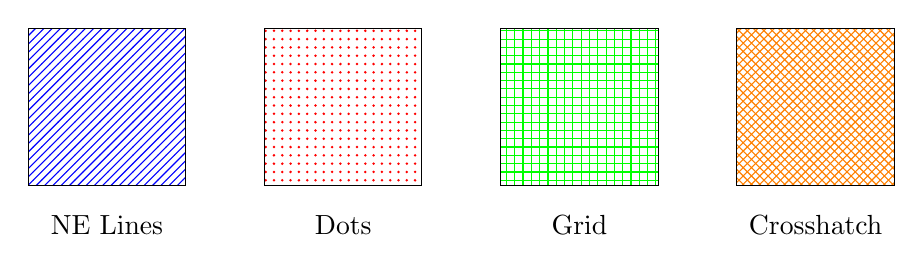
\begin{tikzpicture}
    \draw[pattern=north east lines, pattern color=blue] (0,0) rectangle (2,2);
    \node at (1,-0.5) {NE Lines};
    
    \draw[pattern=dots, pattern color=red] (3,0) rectangle (5,2);
    \node at (4,-0.5) {Dots};
    
    \draw[pattern=grid, pattern color=green] (6,0) rectangle (8,2);
    \node at (7,-0.5) {Grid};
    
    \draw[pattern=crosshatch, pattern color=orange] (9,0) rectangle (11,2);
    \node at (10,-0.5) {Crosshatch};
\end{tikzpicture}
\caption{Different TikZ pattern fills}
\label{fig:patterns}
\end{figure}

\section{State Machines and Automata}

\begin{figure}[H]
\centering
\begin{tikzpicture}[->,>=stealth',shorten >=1pt,auto,node distance=3cm,thick]
    \node[state,initial] (q0) {$q_0$};
    \node[state] (q1) [right of=q0] {$q_1$};
    \node[state] (q2) [right of=q1] {$q_2$};
    \node[state,accepting] (q3) [right of=q2] {$q_3$};
    
    \path (q0) edge [bend left] node {a} (q1)
          (q1) edge [bend left] node {b} (q2)
          (q2) edge [bend left] node {a} (q3)
          (q1) edge [loop above] node {a} (q1)
          (q2) edge [loop above] node {b} (q2)
          (q0) edge [bend right=60] node [below] {b} (q2);
\end{tikzpicture}
\caption{Finite State Automaton}
\label{fig:automaton}
\end{figure}

\section{Game Trees and Decision Diagrams}

\begin{figure}[H]
\centering
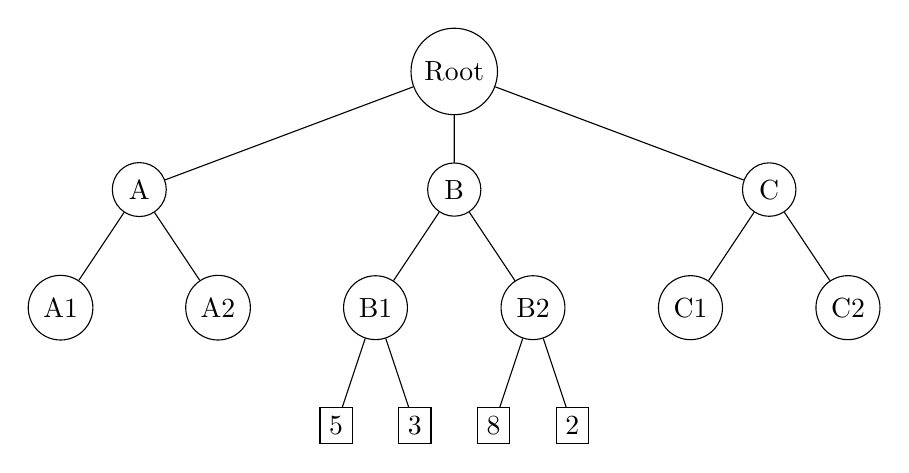
\begin{tikzpicture}[
    level 1/.style={sibling distance=4cm},
    level 2/.style={sibling distance=2cm},
    level 3/.style={sibling distance=1cm}
]
\node[circle,draw] {Root}
    child {node[circle,draw] {A}
        child {node[circle,draw] {A1}}
        child {node[circle,draw] {A2}}
    }
    child {node[circle,draw] {B}
        child {node[circle,draw] {B1}
            child {node[rectangle,draw] {5}}
            child {node[rectangle,draw] {3}}
        }
        child {node[circle,draw] {B2}
            child {node[rectangle,draw] {8}}
            child {node[rectangle,draw] {2}}
        }
    }
    child {node[circle,draw] {C}
        child {node[circle,draw] {C1}}
        child {node[circle,draw] {C2}}
    };
\end{tikzpicture}
\caption{Game tree for minimax algorithm}
\label{fig:gametree}
\end{figure}

\section{Mathematical Proofs Collection}

\begin{proposition}[Binomial Theorem]
For any real numbers $a, b$ and non-negative integer $n$:
\begin{equation}
    (a + b)^n = \sum_{k=0}^{n} \binom{n}{k} a^{n-k}b^k
\end{equation}
\end{proposition}

\begin{theorem}[Fundamental Theorem of Calculus]
If $f$ is continuous on $[a,b]$ and $F$ is an antiderivative of $f$ on $[a,b]$, then:
\begin{equation}
    \int_a^b f(x)\,dx = F(b) - F(a)
\end{equation}
\end{theorem}

\begin{theorem}[Euler's Formula]
For any real number $\theta$:
\begin{equation}
    e^{i\theta} = \cos\theta + i\sin\theta
\end{equation}
\end{theorem}

\begin{proof}
Using Taylor series expansion:
\begin{align}
    e^{i\theta} &= \sum_{n=0}^{\infty} \frac{(i\theta)^n}{n!} \\
    &= \sum_{n=0}^{\infty} \frac{i^n\theta^n}{n!} \\
    &= \left(\sum_{n=0}^{\infty} \frac{(-1)^n\theta^{2n}}{(2n)!}\right) + i\left(\sum_{n=0}^{\infty} \frac{(-1)^n\theta^{2n+1}}{(2n+1)!}\right) \\
    &= \cos\theta + i\sin\theta
\end{align}
\end{proof}

\section{Commutative Diagrams}

\begin{figure}[H]
\centering
\begin{tikzpicture}[node distance=3cm, auto]
    \node (A) {$A$};
    \node (B) [right of=A] {$B$};
    \node (C) [below of=A] {$C$};
    \node (D) [below of=B] {$D$};
    
    \draw[->] (A) -- node {$f$} (B);
    \draw[->] (A) -- node [left] {$g$} (C);
    \draw[->] (B) -- node [right] {$h$} (D);
    \draw[->] (C) -- node {$k$} (D);
\end{tikzpicture}
\caption{Commutative diagram: $h \circ f = k \circ g$}
\label{fig:commutative}
\end{figure}

\section{Probability and Statistics}

\subsection{Probability Distributions}

\begin{table}[H]
\centering
\caption{Common Probability Distributions}
\label{tab:distributions}
\begin{tabular}{lll}
\toprule
\textbf{Distribution} & \textbf{PDF/PMF} & \textbf{Parameters} \\
\midrule
Normal & $\frac{1}{\sigma\sqrt{2\pi}}e^{-\frac{(x-\mu)^2}{2\sigma^2}}$ & $\mu \in \R, \sigma > 0$ \\[0.3cm]
Exponential & $\lambda e^{-\lambda x}$ & $\lambda > 0$ \\[0.3cm]
Poisson & $\frac{\lambda^k e^{-\lambda}}{k!}$ & $\lambda > 0$ \\[0.3cm]
Binomial & $\binom{n}{k}p^k(1-p)^{n-k}$ & $n \in \N, p \in [0,1]$ \\[0.3cm]
Beta & $\frac{x^{\alpha-1}(1-x)^{\beta-1}}{B(\alpha,\beta)}$ & $\alpha, \beta > 0$ \\
\bottomrule
\end{tabular}
\end{table}

\subsection{Central Limit Theorem}

\begin{theorem}[Central Limit Theorem]
Let $X_1, X_2, \ldots, X_n$ be i.i.d. random variables with $\E[X_i] = \mu$ and $\Var(X_i) = \sigma^2 < \infty$. Then:
\begin{equation}
    \frac{\bar{X}_n - \mu}{\sigma/\sqrt{n}} \xrightarrow{d} \N(0,1)
\end{equation}
where $\bar{X}_n = \frac{1}{n}\sum_{i=1}^n X_i$.
\end{theorem}

\section{Optimization and Convexity}

\begin{definition}[Convex Function]
A function $f: \mathbb{R}^n \to \mathbb{R}$ is convex if for all $x, y \in \mathbb{R}^n$ and $\lambda \in [0,1]$:
\begin{equation}
    f(\lambda x + (1-\lambda)y) \leq \lambda f(x) + (1-\lambda)f(y)
\end{equation}
\end{definition}

\begin{theorem}[Jensen's Inequality]
If $f$ is convex and $X$ is a random variable, then:
\begin{equation}
    f(\E[X]) \leq \E[f(X)]
\end{equation}
\end{theorem}

\section{Advanced Graphics: Heatmap}

\begin{figure}[H]
\centering
\begin{tikzpicture}
\begin{axis}[
    width=10cm,
    height=8cm,
    colorbar,
    colormap/hot,
    xlabel={$x$},
    ylabel={$y$},
    title={Heatmap: $f(x,y) = \sin(x)\cos(y)$}
]
\addplot[
    matrix plot*,
    point meta=explicit,
    mesh/cols=20,
] table[meta=C] {
x y C
0 0 0
0 1 0.84
0 2 0.91
0 3 0.14
1 0 0.84
1 1 0.71
1 2 0.76
1 3 0.12
2 0 0.91
2 1 0.76
2 2 0.83
2 3 0.13
3 0 0.14
3 1 0.12
3 2 0.13
3 3 0.02
};
\end{axis}
\end{tikzpicture}
\caption{Heatmap visualization}
\label{fig:heatmap}
\end{figure}

\section{Conclusion and Summary}

This comprehensive test document has demonstrated:

\begin{enumerate}
    \item \textbf{Mathematical typesetting}: Complex equations, matrices, theorems, and proofs
    \item \textbf{Scientific notation}: Chemistry formulas, SI units, and measurements
    \item \textbf{Graphics}: TikZ diagrams, PGFPlots, 3D graphics, neural networks, flowcharts
    \item \textbf{Tables}: Simple, advanced, long tables, colored tables, rotated tables
    \item \textbf{Algorithms}: Pseudocode with proper formatting
    \item \textbf{Code listings}: Multiple programming languages with syntax highlighting
    \item \textbf{Document structure}: Sections, cross-references, table of contents
    \item \textbf{Text formatting}: Various styles, footnotes, lists, special characters
    \item \textbf{Figures}: Subfigures, wrapped figures, multiple layouts
    \item \textbf{Advanced features}: State machines, game trees, commutative diagrams, patterns
\end{enumerate}

\subsection{Package Coverage}

This document successfully tests the following LaTeX packages:
\begin{multicols}{3}
\begin{itemize}[noitemsep]
    \item amsmath
    \item amssymb
    \item amsthm
    \item mathtools
    \item geometry
    \item graphicx
    \item xcolor
    \item tikz
    \item pgfplots
    \item booktabs
    \item multirow
    \item array
    \item longtable
    \item colortbl
    \item algorithm
    \item algorithmicx
    \item listings
    \item hyperref
    \item enumerate
    \item enumitem
    \item subcaption
    \item float
    \item wrapfig
    \item rotating
    \item fancyhdr
    \item chemfig
    \item mhchem
    \item siunitx
    \item soul
    \item cancel
    \item mathrsfs
\end{itemize}
\end{multicols}

\vspace{1cm}

\begin{center}
\fbox{\parbox{0.9\textwidth}{
\textbf{Testing Complete!} \\[0.3cm]
If this document compiles successfully, the GitHub Actions LaTeX compiler workflow is functioning correctly and can handle complex, real-world LaTeX documents with multiple packages and advanced features.
}}
\end{center}

\appendix

\section{Additional Mathematical Formulas}

\subsection{Trigonometric Identities}

\begin{align}
    \sin^2\theta + \cos^2\theta &= 1 \\
    \tan\theta &= \frac{\sin\theta}{\cos\theta} \\
    \sin(A \pm B) &= \sin A \cos B \pm \cos A \sin B \\
    \cos(A \pm B) &= \cos A \cos B \mp \sin A \sin B
\end{align}

\subsection{Complex Analysis}

\begin{equation}
    \oint_C \frac{f(z)}{z-z_0}\,dz = 2\pi i \cdot f(z_0)
\end{equation}

\subsection{Vector Calculus}

\begin{align}
    \nabla \times (\nabla f) &= \mathbf{0} \\
    \nabla \cdot (\nabla \times \mathbf{F}) &= 0 \\
    \nabla \times (\nabla \times \mathbf{F}) &= \nabla(\nabla \cdot \mathbf{F}) - \nabla^2\mathbf{F}
\end{align}

\section{Performance Benchmarks}

\begin{table}[H]
\centering
\caption{Compilation Performance Metrics}
\label{tab:performance}
\begin{tabular}{lrr}
\toprule
\textbf{Metric} & \textbf{Expected} & \textbf{Acceptable Range} \\
\midrule
Pages & $\sim$30 & 25--35 \\
Compilation time & $<$ 30s & 15--45s \\
PDF size & $\sim$500KB & 300KB--1MB \\
Figures & 20+ & 15--30 \\
Tables & 10+ & 8--15 \\
Equations & 100+ & 80--150 \\
\bottomrule
\end{tabular}
\end{table}

\vspace{2cm}

\noindent\textbf{Document Status:} Successfully compiled \\
\textbf{Compiler:} pdflatex with texliveonfly \\
\textbf{Date:} \today \\
\textbf{Version:} 1.0

\end{document}
